\subsection{Ride Manager}\label{comp:rideManager}
\subsubsection{Internal Components}
The Ride Manager is responsible for the communication with passengers, and for the management of the life cycle of requests and reservations. Internally it is composed of the following components each with a precise job:
\begin{itemize}
	\item \textit{RideDispatcher}: it exposes the interfaces for external calls and dispatches them to the right subcomponent depending on the nature of the call.	
	\item \textit{RequestHandler}: for every request it receives, it first checks for the validity of the location, then if this is valid it stores the request through the Data Access. Right after that, it forwards the request to the requestQueueManager. If the requestQueueManager finds a taxi driver, the handler computes the waiting time through the Geographic Engine, and returns to the passenger an affirmative response with the info, otherwise a negative response. The method for making a request is synchronous, this means that the passenger gui will wait until it gets a response by the server.
	\item \textit{ReservationHandler}: for every reservation it receives, it first check for the validity of the location, then if this is valid it stores the reservation through the Data Access. It then waits until 10 minutes before the meeting time and then it forwards the reservation (in the form of a request) to the requestQueueManager (for further details about the algorithm that manages the wait for every reservation see \ref{alg:reservationHandler}). It keeps forwarding the reservation until it gets a taxi driver, then it computes the waiting time through the Geographic Engine, and then sends an affirmative message to the passenger with the info. The method for making a reservation is carried out in two phases. The first is synchronous, this means that the passenger gui will wait for the affirmative response after submitting the reservation. The second is synchronous, this means that the gui will not wait for a response from the server but the server will just send a message with the info when needed.
	\item \textit{RequestQueueManager}: it is in charge of calling the  provideTaxi method of the Taxi Manager component. It is separated from the two handlers because the idea behind seeking a taxi is the same between requests and reservations and in future possibly it can also add some priority policies.
\end{itemize}
\begin{figure}[H]
	\centering
	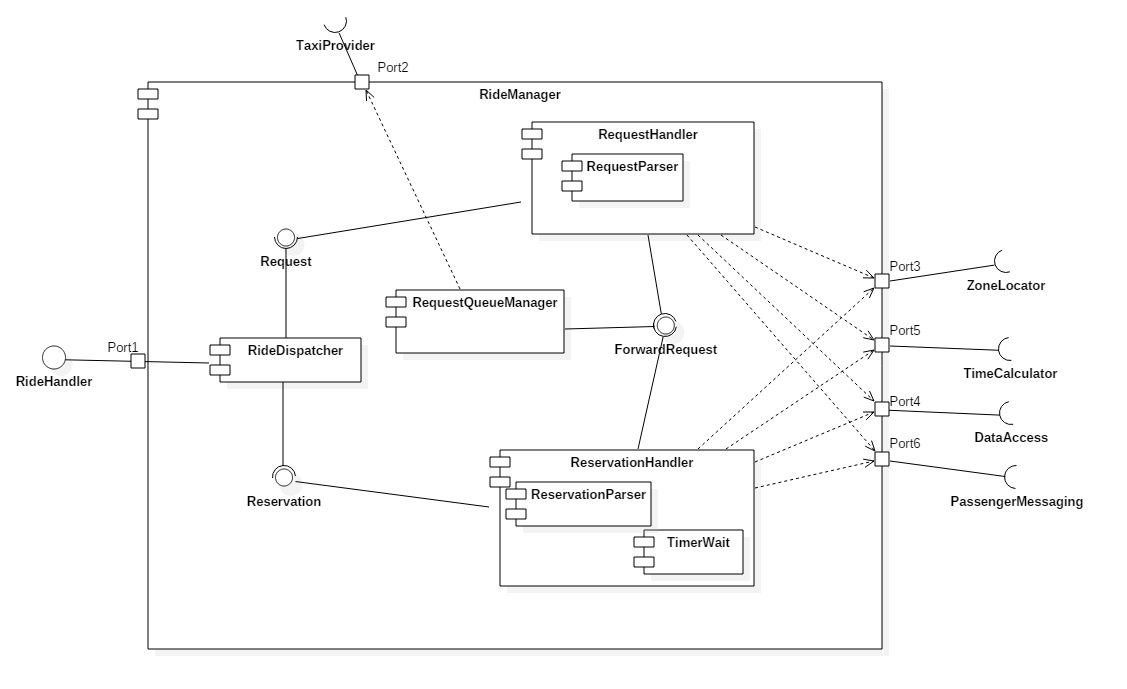
\includegraphics[trim=50 0 0 0,scale=0.45]{../"Analysis Documents"/components/ridemanager}
	\label{fig:rideHandler}
	\caption{Ride Handler}
\end{figure}
\subsubsection{Provided interfaces}
\begin{table}[H]
\begin{longtable}{| p{0.3\textwidth} | p{0.3\textwidth} | p{0.4\textwidth} |}
\hline
 \textbf{Provided Interface} & \textbf{Dedicated user} & \textbf{Description} \\ \hline
RideHandler & The Passenger's application and the relative web application & Login, logout, registration and deletion of the account \\ \hline
\end{longtable}
\caption{Ride Handler: provided interfaces}
\label{tab:rideHandler:providedInterfaces}
\end{table}
\subsubsection{Required interfaces}
\begin{table}[H]
\begin{longtable}{| l | p{.80\textwidth} |}
\hline
 \textbf{Required Interface} & \textbf{Description and usage} \\ \hline
DataAccess & Access to the data layer in order to 
			\begin{itemize}
				\item Store data of the request
				\item Store data of the reservation
				\item Retrieve reservations in order to forward them to the TaxiManager
			\end{itemize} \\ \hline
Zone Locator & Check the correctness of the location data provided by the user \\ \hline
Time Calculator & Calculate the approximative waiting time \\ \hline
TaxiProvider & Retrieve a taxi who accepted the request/reservation or an error message saying the nature of the problem. \\ \hline
PassengerMessaging & Sends to the passenger the info for the taxi driver who is going to serve a reservation. \\ \hline
\end{longtable}
\caption{Ride Handler: required interfaces}
\label{tab:rideHandler:requiredInterfaces}
\end{table}
